% =====================================================================
%  CAPÍTULO III — ANÁLISE E DISCUSSÃO DOS DADOS
%
%  Revisado em 2026-10-05: texto corrido, sem negrito no meio do texto,
%  gráficos como "Gráfico" (Manual FATEC-ID, item 3), tabelas em corpo 10,
%  e a seção de significância (testes pareados), que faltava.
%  Versão anterior em notas/rascunhos/antes_revisao_2026-10-05/.
%
%  Números refeitos em 2026-10-06 com o EA corrigido (notas/INCERTEZAS.md,
%  itens 43 a 51). Versão anterior em notas/rascunhos/antes_refacao_2026-10-06/.
%
%  Procedência (todo número desta página sai destes arquivos; R = 
%  dados/resultados/refeito_2026-10-05/):
%   - Tabela replica: dados/FONTES.md item 7 (Almeida) e
%     dados/resultados/replica_almeida_2026-09-28/ (só médias móveis, não mudou)
%   - Tabela condições originais: R/testes/metricas_cenA_1316_* (idênticos aos de
%     cenario_almeida_2026-09-30) e replica_almeida_2026-09-28/metricas_fl13of.csv
%   - Tabela principal: R/testes/metricas_R6_*.csv (ret_selic, cagr_selic_camada,
%     sharpe, sharpe_p, dd_selic, saidas); Calmar da calibração em R/escolhas/r6_C4.txt
%   - Tabela janelas: R/testes/metricas_R3_T*.csv; 2008 em R/testes/anual_R3_T1.csv
%   - Tabela ativos e venda a descoberto: R/analise_grades.txt (blocos 2 e 3)
%   - Tabela longo: R/testes/metricas_L1_*.csv e metricas_L2_*.csv;
%     concentração em R/testes/anual_L1_escolhas.csv (parcela do retorno em log)
%   - Tabela significância e × médias móveis: R/testes/comparacoes.csv
%   - Tabela mecanismo: taxa_acerto de R6_ARIMA e R6_GS; cenA_1316 (vetos/sinais)
%   - 03/04/2020: R/traco_demo/traco_demo_GARCH.csv (prev_dif, vol_prevista, limiar)
%   - Persistência (limitações): R/analise_grades.txt, bloco 5, PETR4 só compra
%   - Proventos (limitações, revisão de 2026-10-12): R/testes/metricas_R6_*.csv,
%     colunas bh_total (726,5%), ret_completo (MM 396,1%, GS 353,4%) e
%     dd_completo; pares com GARCH × gêmea com proventos: metricas_R3_*, R6_*,
%     L1_*, L2_* (ret_completo, dd_completo). Proventos: dados/series/proventos_PETR4.csv
%   - × médias móveis, 12 comparações (T1, T2, T3 e 2017-2024): R/testes/comparacoes.csv
% =====================================================================
\setdiv{CAPÍTULO III}
\chapter{Análise e discussão dos dados}

Este capítulo apresenta e discute os resultados dos experimentos. Começa pela
reprodução do estudo de \citeonline{almeida2016}, que garante que a estratégia
usada como termo de comparação é de fato a do autor. Em seguida, apresenta o
experimento principal, examina se o comportamento observado se repete em outros
períodos e em outros ativos e avalia a significância estatística das diferenças.
Por fim, discute o mecanismo que produz o efeito observado e as limitações dos
resultados.

\section{Reprodução e comparação com o estudo de referência}

Para que a comparação com \citeonline{almeida2016} fosse legítima, era necessário
verificar que a estratégia de médias móveis reimplementada se comporta como a
original. Os testes do autor foram repetidos com as mesmas datas, o mesmo capital
de R\$ 50 mil, as mesmas médias de 10 e 20 períodos, sem custos e com operações
de compra e venda, como declarado em seu trabalho.

Duas condições, porém, não puderam ser repetidas exatamente. A primeira é a série
de preços. O autor utilizou o histórico fornecido pela corretora por meio do
próprio MetaTrader 5, sem informar se e como os preços foram ajustados, enquanto
este trabalho utilizou o arquivo COTAHIST da B3 corrigido apenas pelos
desdobramentos, conforme descrito na seção~\ref{sec:coleta}. A segunda é o volume. O autor
declara mil ações para o teste de 2013 a 2016, mas não informa o volume dos
testes de crise. Como ele menciona cem ações como volume mínimo e afirma que o
volume de mil foi adotado no período de 2013 a 2016, a reprodução dos testes de
crise utilizou cem ações. Além disso, o código publicado no anexo do trabalho
traz ligada uma opção de gestão de capital cujo arquivo não foi incluído, de modo
que não é possível saber se o volume dele era de fato fixo. Os resultados estão
na Tabela~\ref{tab:replica}.

\begin{table}[htb]
\centering
\caption{Reprodução dos testes de Almeida (2016)}
\label{tab:replica}
\fontsize{10}{12}\selectfont
\begin{tabular}{l|c|c|c|c}
\hline
& \multicolumn{2}{c|}{Almeida (2016)} & \multicolumn{2}{c}{Reprodução} \\
\cline{2-3}
\cline{4-5}
Período & Operações & Resultado & Operações & Resultado \\
\hline
2013 a 2016 & 38 & +R\$ 10.430 & 37 & +R\$ 10.050 \\
\hline
2008 a 2010 & 37 & $-$R\$ 1.595 & 38 & $-$R\$ 575 \\
\hline
2007 a 2011 & 52 & $-$R\$ 2.542 & 63 & $-$R\$ 1.274 \\
\hline
\end{tabular}
\fonte{Elaboração própria e \citeonline{almeida2016}.}
\nota{Médias móveis simples de 10 e 20 períodos, capital de R\$ 50 mil, sem custos, compra e venda. Volume de mil ações em 2013 a 2016 e de cem ações nos testes de crise.}
\end{table}

No período fora de crise, a reprodução difere do original em uma operação e em
3,6\% do lucro, o que indica que a lógica da estratégia foi reproduzida. No
subperíodo de 2008 a 2010, a quantidade de operações praticamente coincide, mas
os valores em reais divergem, e no período completo de crise coincidem apenas o
sinal e a ordem de grandeza do resultado.

A divergência em reais tem uma explicação provável. O resultado em reais de uma
estratégia com lote fixo é proporcional ao nível de preço da série, de modo que
uma série vinte por cento mais baixa produz variações em reais vinte por cento
menores, ainda que os retornos percentuais sejam idênticos. Uma verificação com a
série ajustada também por proventos, obtidos do Yahoo Finance, deslocou o lucro bruto de 2008 a 2010 na
direção do valor relatado pelo autor, o que indica que boa parte da diferença
decorre do critério de ajuste da série. A diferença na quantidade de operações
de 2007 a 2011, porém, não foi explicada. O mesmo ajuste por proventos afastou a
contagem do valor do autor, em vez de aproximá-la. Restam duas possibilidades que
não podem ser verificadas sem os dados originais: a série usada pelo autor
diferia da série da bolsa também na forma, e não só no nível, ou a simulação dele,
feita negócio a negócio, gerou entradas diferentes das obtidas aqui com preços de
abertura, já que o arquivo da bolsa traz apenas o resumo diário de cada pregão.

Conclui-se que a reprodução confirma o comportamento do algoritmo de referência,
mas não os seus valores financeiros. Isso basta para o propósito desta etapa, que
é garantir que a estratégia usada como termo de comparação nas seções seguintes é
de fato a de \citeonline{almeida2016}. A reprodução exata dos valores
dependeria do critério de ajuste da série e do volume dos testes de crise, que o
estudo original não registra.

Validada a reimplementação, os modelos deste trabalho foram executados nas
mesmas condições declaradas por \citeonline{almeida2016} para o período de 2013 a 2016,
com capital de R\$ 50 mil, volume fixo de mil ações, sem custos e com operações
de compra e venda. Para o ARIMA-GARCH foi usada a configuração padrão do
\textit{Expert Advisor}, com o GARCH como filtro, limiar no percentil 50 da
volatilidade estimada e janela de 120 pregões. A Tabela~\ref{tab:cenario-almeida}
apresenta o resultado.

\begin{table}[htb]
\centering
\caption{Comparação nas condições originais, 2013 a 2016}
\label{tab:cenario-almeida}
\fontsize{10}{12}\selectfont
\begin{tabular}{l|c|c|c}
\hline
Algoritmo & Operações & Resultado & Queda máx. \\
\hline
Médias móveis, relatado por Almeida & 38 & +R\$ 10.430 & -- \\
\hline
Médias móveis, reproduzido & 37 & +R\$ 10.050 & 15,0\% \\
\hline
ARIMA isolado & 397 & $-$R\$ 8.100 & 30,9\% \\
\hline
ARIMA-GARCH & 173 & +R\$ 24.020 & 8,7\% \\
\hline
\end{tabular}
\fonte{Elaboração própria e \citeonline{almeida2016}.}
\nota{Sem custos de execução, conforme o estudo original.}
\end{table}

Nas mesmas condições em que o estudo de referência obteve lucro de R\$ 10.430,
equivalente a 20,9\% do capital, o ARIMA-GARCH obteve R\$ 24.020, ou 48,0\%, com
queda máxima de 8,7\%, contra 15,0\% das médias móveis reproduzidas. A linha
reproduzida é o que torna a comparação interpretável. A diferença entre as duas
primeiras linhas decorre dos dados, e a diferença entre a segunda e a quarta
decorre do modelo. Cabe registrar que, nessas condições, o ARIMA isolado realizou
397 operações, contra 173 do ARIMA-GARCH e 37 das médias móveis. Como o estudo
original não considera custos de execução, esse giro não tem custo na simulação,
o que não ocorreria na prática.

\section{Resultado principal: teste fora da amostra}

O experimento central testou o ARIMA-GARCH no período de 2017 a 2024, seguindo o
plano da seção~\ref{sec:protocolo}. As configurações foram escolhidas nos três
anos anteriores, de 2014 a 2016, e cada uma foi comparada à sua gêmea, com o mesmo
ARIMA e o GARCH desligado. Os resultados estão na Tabela~\ref{tab:principal}.

\begin{table}[htb]
\centering
\caption{Desempenho no período de teste, 2017 a 2024}
\label{tab:principal}
\fontsize{10}{12}\selectfont
\begin{tabular}{l|c|c|c|c|c|c}
\hline
Algoritmo & Retorno & Ao ano & Sharpe & $p$ & Queda máx. & Oper. \\
\hline
ARIMA-GARCH, escolha por Sharpe & +273,8\% & 18,2\% & 0,49 & 0,085 & 26,1\% & 238 \\
\hline
\quad gêmea sem GARCH           & +114,6\% & 10,2\% & 0,22 & 0,268 & 40,6\% & 244 \\
\hline
ARIMA-GARCH, escolha por Calmar & +114,1\% & 10,2\% & 0,19 & 0,295 & 38,1\% & 223 \\
\hline
\quad gêmea sem GARCH           & $-$46,5\% & $-$7,6\% & $-$0,34 & 0,831 & 78,4\% & 469 \\
\hline
Médias móveis de Almeida        & +90,4\%  & 8,5\%  & 0,17 & 0,319 & 36,7\% & 56 \\
\hline
Taxa Selic                      & +86,1\%  & 8,2\%  & -- & -- & -- & -- \\
\hline
Compra e manutenção da PETR4    & +143,6\% & 12,0\% & -- & -- & -- & -- \\
\hline
\end{tabular}
\fonte{Elaboração própria.}
\nota{Valores com custos de execução e remuneração do caixa pela Selic, sem proventos. A compra e manutenção é medida pela variação do preço. O valor-p refere-se à hipótese de índice de Sharpe positivo. O ARIMA isolado escolhido na calibração coincidiu com a gêmea da escolha por Sharpe.}
\end{table}

Nos dois pares, a versão com GARCH obteve retorno maior e queda máxima menor que
a sua gêmea. Na configuração escolhida por Sharpe, o retorno passou de 114,6\%
para 273,8\%, e a queda máxima caiu de 40,6\% para 26,1\%. Na escolhida por Calmar,
a diferença foi maior, de um prejuízo de 46,5\% para um lucro de 114,1\%, com a
queda máxima caindo de 78,4\% para 38,1\%. Como cada par parte do mesmo modelo de
previsão e difere apenas na presença do GARCH, a diferença dentro do par pode ser
atribuída ao componente de volatilidade.

A configuração escolhida por Sharpe também teve retorno maior que o das médias
móveis de \citeonline{almeida2016}, que o da Selic e que o da compra e manutenção
do ativo no mesmo período. Essas diferenças, porém, não são estatisticamente
significativas, como se discute na seção~\ref{sec:significancia}, e dependem de
os proventos ficarem fora da medida, como se discute nas limitações. Por isso o
resultado deve ser lido como retorno superior no período observado, e não como
superioridade demonstrada.

O critério de escolha por Calmar não se manteve do período de calibração para o
de teste. A configuração escolhida por esse critério tinha, na calibração, índice
de Calmar de 2,83 e queda máxima de 8,4\%, e no teste apresentou 0,27 e 38,1\%.

\section{Robustez entre períodos e entre ativos}

O mesmo procedimento foi aplicado a outras três janelas, cada uma com escolha
própria, para verificar se o comportamento observado depende do período. A
Tabela~\ref{tab:janelas} resume os resultados.

\begin{table}[htb]
\centering
\caption{Desempenho por janela de teste}
\label{tab:janelas}
\fontsize{10}{12}\selectfont
\begin{tabular}{l|l|c|c|c}
\hline
Janela & Algoritmo & Retorno & Queda máx. & Sharpe ($p$) \\
\hline
\multirow{4}{*}{2007 a 2011} & ARIMA-GARCH & +28,7\% & 13,3\% & $-$0,47 (0,85) \\
\cline{2-5}
 & gêmea sem GARCH & +19,8\% & 35,1\% & $-$0,10 (0,59) \\
\cline{2-5}
 & ARIMA isolado & $-$2,1\% & 44,3\% & $-$0,26 (0,72) \\
\cline{2-5}
 & Médias móveis & $-$11,6\% & 57,5\% & $-$0,31 (0,76) \\
\hline
\multirow{5}{*}{2013 a 2016} & ARIMA-GARCH, por Sharpe & +15,8\% & 17,7\% & $-$0,44 (0,81) \\
\cline{2-5}
 & ARIMA-GARCH, por Calmar & +34,0\% & 6,8\% & $-$0,46 (0,82) \\
\cline{2-5}
 & gêmea sem GARCH & $-$3,7\% & 50,9\% & $-$0,16 (0,63) \\
\cline{2-5}
 & ARIMA isolado & $-$30,5\% & 51,9\% & $-$0,35 (0,75) \\
\cline{2-5}
 & Médias móveis & +150,9\% & 38,4\% & 0,50 (0,16) \\
\hline
\multirow{4}{*}{2025 a 2026} & ARIMA-GARCH, por Sharpe & $-$0,4\% & 13,7\% & $-$0,94 (0,89) \\
\cline{2-5}
 & ARIMA-GARCH, por Calmar & +9,6\% & 8,2\% & $-$0,82 (0,86) \\
\cline{2-5}
 & ARIMA isolado & +24,1\% & 19,0\% & 0,08 (0,46) \\
\cline{2-5}
 & Médias móveis & +31,3\% & 28,2\% & 0,23 (0,38) \\
\hline
\end{tabular}
\fonte{Elaboração própria.}
\nota{Em 2007 a 2011, os dois critérios escolheram a mesma configuração. Em 2013 a 2016, as duas escolhas têm a mesma gêmea. Em 2025 e 2026, a gêmea das duas escolhas é o próprio ARIMA isolado. Referências: Selic de +68,1\%, +53,9\% e +25,7\%, e PETR4, pela variação do preço, de $-$14,0\%, $-$25,6\% e +33,2\%, respectivamente.}
\end{table}

O padrão que se repete é o da redução de risco. Em todas as janelas, a menor
queda máxima pertence a uma variante com GARCH, e nas duas janelas de turbulência
a diferença é grande. Em 2007 a 2011, a queda máxima foi de 13,3\%, contra 44,3\%
do ARIMA isolado e 57,5\% das médias móveis. Em 2013 a 2016, foi de 6,8\%, contra
51,9\% e 38,4\%.

O retorno, ao contrário, não segue um padrão. Em 2007 a 2011, a variante com
GARCH teve o maior retorno entre os algoritmos, mas em 2013 a 2016 e em 2025 e
2026 as médias móveis superaram os modelos estatísticos, e no período mais
recente o ARIMA isolado também rendeu mais que as variantes com GARCH.

O ano de 2008 ilustra o comportamento em uma crise. Enquanto a PETR4 recuou
47,3\% no ano, o ARIMA-GARCH encerrou com ganho de 5,0\%, contra perdas de 24,8\%
do ARIMA isolado e de 36,6\% das médias móveis. O Gráfico~\ref{gra:curva-t1}
mostra a evolução do patrimônio de cada algoritmo entre 2007 e 2011, e o
Gráfico~\ref{gra:anual-t1}, o retorno de cada ano.

\begin{grafico}[htb]
\centering
\caption{Evolução do patrimônio e da queda acumulada, 2007 a 2011}
\label{gra:curva-t1}
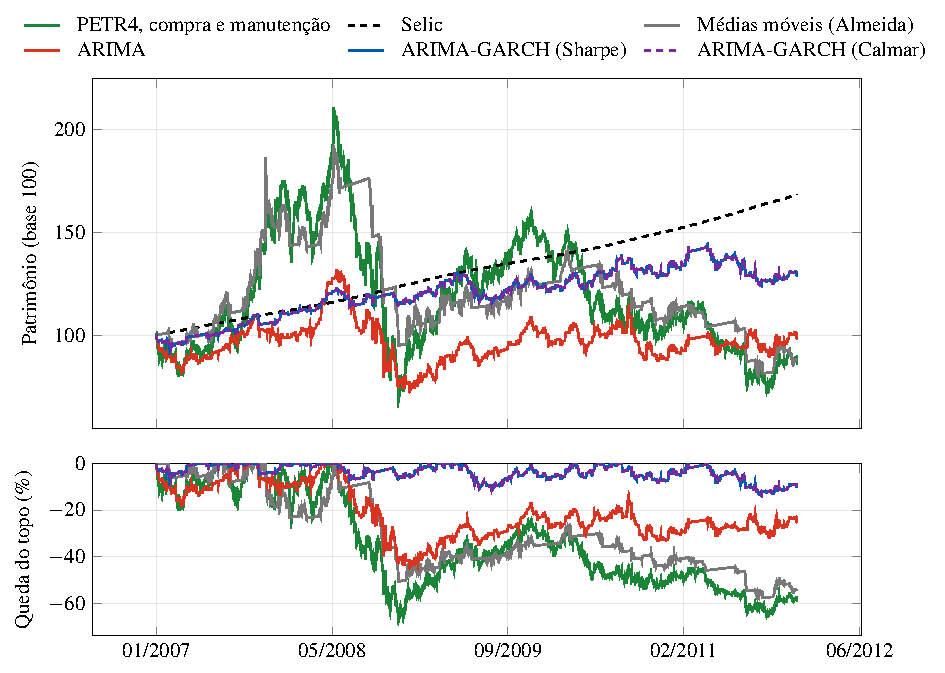
\includegraphics{../graficos/rodada3/curva_T1.pdf}
\fonte{Elaboração própria.}
\end{grafico}

\begin{grafico}[htb]
\centering
\caption{Retorno por ano, 2007 a 2011}
\label{gra:anual-t1}
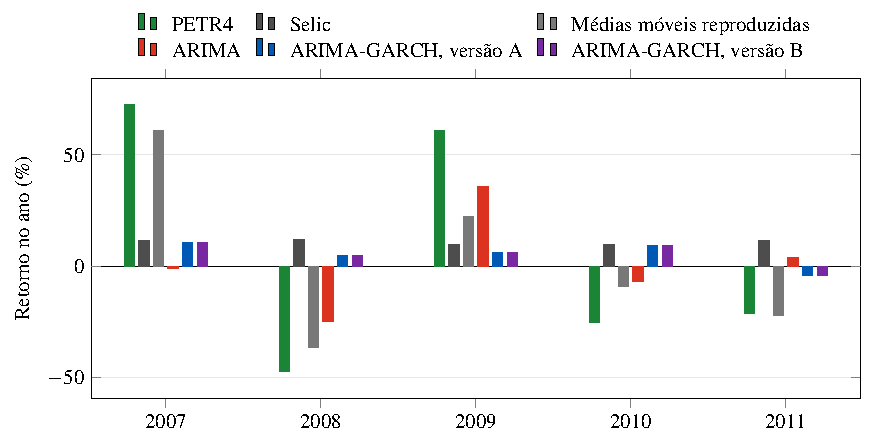
\includegraphics{../graficos/rodada3/anual_T1.pdf}
\fonte{Elaboração própria.}
\end{grafico}

Para verificar se o efeito é específico da PETR4, o procedimento foi repetido nas
ações VALE3, USIM5 e POMO4, totalizando 16.512 simulações. A análise foi feita por
pares. Cada configuração com GARCH foi comparada à sua gêmea, e contou-se em que
proporção dos pares o GARCH reduziu a queda máxima. A Tabela~\ref{tab:ativos}
apresenta o resultado para as variantes que limitam a exposição, isto é, as que
dimensionam a entrada pela volatilidade prevista ou encerram a posição no veto.

\begin{table}[htb]
\centering
\caption{Efeito do GARCH sobre o risco nos quatro ativos}
\label{tab:ativos}
\fontsize{10}{12}\selectfont
\begin{tabular}{l|c|c|c}
\hline
& 2007 a 2011 & 2013 a 2016 & 2025 a 2026 \\
\hline
Pares em que reduziu a queda máxima & 85\% a 93\% & 92\% a 98\% & 52\% a 96\% \\
\hline
Variação da queda máxima (p.p.) & $-$17 a $-$29 & $-$20 a $-$40 & 0 a $-$22 \\
\hline
Variação do retorno (p.p.) & +7 a +27 & +29 a +41 & +2 a +16 \\
\hline
Variação do índice de Sharpe & $-$0,08 a $-$0,02 & $-$0,08 a +0,05 & $-$0,12 a +0,10 \\
\hline
\end{tabular}
\fonte{Elaboração própria.}
\nota{As faixas correspondem aos quatro ativos. As variações são medianas das diferenças entre cada configuração com GARCH e sua gêmea.}
\end{table}

O efeito sobre o risco se confirma nos quatro ativos, com uma condição. Ele
pertence às variantes que limitam a exposição. As variantes que apenas impedem
novas entradas, mantendo a posição já aberta, reduziram a queda máxima em 23\% a
67\% dos pares, conforme o ativo e o período, com variação mediana próxima de zero.
Já o efeito sobre o índice de Sharpe ficou próximo de zero em todos os casos.

As mesmas simulações permitiram testar a venda a descoberto, prevista como
possibilidade no início do trabalho. O resultado foi negativo. Em nove dos doze
casos de ativo e período, a mediana do retorno piorou quando se permitiu operar
vendido, em dois melhorou e em um não se alterou, e menos de 1\% das
configurações levou o capital à ruína nas janelas de crise. Com o modelo acertando
a direção em taxa próxima ao acaso, operar nos dois sentidos dobra a exposição ao
erro em vez de aproveitar as quedas.

\section{Horizonte longo}

Também foram testadas configurações fixas, mantidas sem nova escolha ao longo do
tempo, da mesma forma que \citeonline{almeida2016} manteve fixas as suas médias
de 10 e 20 períodos. Foram usadas as duas configurações escolhidas na calibração
de 2010 a 2012, pelos critérios de Sharpe e de Calmar. As duas usam o GARCH como
filtro e para dimensionar a entrada, encerram a posição no veto e diferem apenas
na volatilidade de referência para o tamanho da posição, de 2\% e de 1\% ao dia.
Elas foram aplicadas ao período mais longo disponível, de 2005 a 2026, e ao
período de 2017 a 2024, sempre ao lado da sua gêmea sem GARCH. Como a calibração
está dentro do primeiro período, ainda que corresponda a apenas três dos vinte e
um anos, o teste de 2017 a 2024, inteiramente posterior a ela, é o mais limpo dos
dois. A Tabela~\ref{tab:longo} apresenta o resultado.

\begin{table}[htb]
\centering
\caption{Desempenho das configurações fixas}
\label{tab:longo}
\fontsize{10}{12}\selectfont
\begin{tabular}{l|l|c|c|c|c}
\hline
Período & Algoritmo & Retorno & Ao ano & Sharpe ($p$) & Queda máx. \\
\hline
\multirow{4}{*}{2005 a 2026} & ARIMA-GARCH, por Sharpe & +602,4\% & 9,6\% & $-$0,01 (0,514) & 29,7\% \\
\cline{2-6}
 & ARIMA-GARCH, por Calmar & +669,9\% & 10,0\% & $-$0,05 (0,600) & 14,2\% \\
\cline{2-6}
 & gêmea sem GARCH & +79,9\% & 2,8\% & $-$0,11 (0,702) & 80,7\% \\
\cline{2-6}
 & Médias móveis de Almeida & +985,2\% & 11,8\% & 0,18 (0,198) & 67,5\% \\
\hline
\multirow{4}{*}{2017 a 2024} & ARIMA-GARCH, por Sharpe & +67,3\% & 6,8\% & 0,01 (0,492) & 28,1\% \\
\cline{2-6}
 & ARIMA-GARCH, por Calmar & +72,9\% & 7,2\% & $-$0,06 (0,572) & 12,6\% \\
\cline{2-6}
 & gêmea sem GARCH & +11,9\% & 1,4\% & $-$0,03 (0,533) & 57,8\% \\
\cline{2-6}
 & Médias móveis de Almeida & +90,4\% & 8,5\% & 0,17 (0,319) & 36,7\% \\
\hline
\end{tabular}
\fonte{Elaboração própria.}
\nota{As duas escolhas têm a mesma gêmea. Selic de +795,8\% (10,8\% ao ano) e +86,1\% (8,2\% ao ano), e compra e manutenção da PETR4, pela variação do preço, de +298,8\% (6,7\% ao ano) e +143,6\% (12,0\% ao ano), respectivamente.}
\end{table}

O resultado mais forte da Tabela~\ref{tab:longo} é a diferença entre o mesmo
ARIMA com e sem o GARCH. Sem o GARCH, o ARIMA rendeu 79,9\% em vinte e um anos e
11,9\% entre 2017 e 2024, com quedas máximas de 80,7\% e 57,8\%. Com o GARCH, a
mesma previsão rendeu 602,4\% e 669,9\% no período longo, com quedas máximas de
29,7\% e 14,2\%, e de 67,3\% a 72,9\% no período de 2017 a 2024, com quedas de
28,1\% e 12,6\%.

Ainda assim, nenhuma das configurações fixas superou a Selic no período longo, e
as médias móveis de \citeonline{almeida2016} tiveram o maior retorno nos dois
períodos, com quedas máximas maiores. O retorno das variantes com GARCH também é
concentrado. Na escolha por Sharpe, os cinco melhores anos respondem por 67,5\%
do retorno acumulado, e um único ano, 2018, por 19,2\%.

\section{Significância das diferenças}
\label{sec:significancia}

As seções anteriores mostram que o GARCH alterou o desempenho do ARIMA em quase
todos os testes. Resta saber se essas diferenças são grandes o bastante para não
serem atribuídas ao acaso. Para isso, cada configuração com GARCH foi comparada à
sua gêmea sobre os mesmos dias, pelo teste de diferença entre índices de Sharpe. A
Tabela~\ref{tab:significancia} reúne as onze comparações realizadas.

\begin{table}[htb]
\centering
\caption{Comparação entre cada configuração com GARCH e sua gêmea}
\label{tab:significancia}
\fontsize{10}{12}\selectfont
\begin{tabular}{l|l|c|c|c}
\hline
Período & Configuração & Sharpe com GARCH & Sharpe da gêmea & $p$ \\
\hline
2007 a 2011 & escolha por Sharpe e por Calmar & $-$0,47 & $-$0,10 & 0,259 \\
\hline
2013 a 2016 & escolha por Sharpe & $-$0,44 & $-$0,16 & 0,540 \\
\hline
2013 a 2016 & escolha por Calmar & $-$0,46 & $-$0,16 & 0,521 \\
\hline
2017 a 2024 & escolha por Sharpe & 0,49 & 0,22 & 0,281 \\
\hline
2017 a 2024 & escolha por Calmar & 0,19 & $-$0,34 & 0,020 \\
\hline
2025 a 2026 & escolha por Sharpe & $-$0,94 & 0,08 & 0,128 \\
\hline
2025 a 2026 & escolha por Calmar & $-$0,82 & 0,08 & 0,179 \\
\hline
2005 a 2026 & escolha por Sharpe, fixa & $-$0,01 & $-$0,11 & 0,587 \\
\hline
2005 a 2026 & escolha por Calmar, fixa & $-$0,05 & $-$0,11 & 0,764 \\
\hline
2017 a 2024 & escolha por Sharpe, fixa & 0,01 & $-$0,03 & 0,907 \\
\hline
2017 a 2024 & escolha por Calmar, fixa & $-$0,06 & $-$0,03 & 0,913 \\
\hline
\end{tabular}
\fonte{Elaboração própria.}
\nota{Teste de diferença entre índices de Sharpe com a correção de Memmel, sobre os retornos diários dos mesmos pregões.}
\end{table}

Em uma das onze comparações, a do período de 2017 a 2024 com a escolha por
Calmar, a versão com GARCH foi significativamente melhor que a gêmea, ao nível de
5\%, e em nenhuma foi significativamente pior. Nas demais, a diferença de índice
de Sharpe não pode ser distinguida do acaso, mesmo quando a diferença de retorno
e de queda máxima é grande.

Há uma razão para isso. O índice de Sharpe deste trabalho é medido em relação à
Selic, e, quando um algoritmo rende menos que ela, o índice é negativo. Nesse
caso, reduzir a oscilação torna o índice ainda mais negativo, mesmo que o retorno
tenha aumentado. Foi o que ocorreu em 2007 a 2011 e em 2013 a 2016. A versão com
GARCH rendeu mais que a gêmea e oscilou bem menos, mas, como as duas ficaram
abaixo da Selic, o índice da versão com GARCH ficou mais negativo. O índice de
Sharpe, portanto, mede a vantagem sobre a Selic, e não a proteção contra quedas,
que aparece na queda máxima.

A mesma análise foi feita entre os modelos deste trabalho e as médias móveis de
\citeonline{almeida2016}, nas doze comparações possíveis entre as quatro janelas de
teste com escolha na calibração, incluído o período de 2017 a 2024, e nenhuma
diferença foi significativa, com valores-p entre 0,11 e 0,95. Os
dados, portanto, permitem afirmar que o GARCH reduziu o risco do ARIMA, mas não
permitem afirmar que o ARIMA-GARCH superou a estratégia de médias móveis.

A comparação com a Selic segue a mesma lógica. Como o índice de Sharpe deste
trabalho é medido em relação à Selic, um índice positivo indica que o algoritmo
rendeu mais que ela, e o valor-p que acompanha cada índice indica se essa vantagem
pode ser distinguida do acaso. Os valores-p das Tabelas~\ref{tab:principal},
\ref{tab:janelas} e~\ref{tab:longo} mostram que, em nenhum dos casos, ela pode. A
configuração principal de 2017 a 2024 rendeu 273,8\% contra 86,1\% da Selic, mas
com valor-p de 0,085. Os algoritmos renderam mais que a Selic em alguns
períodos, mas essa vantagem é compatível com o acaso. É por isso que a Selic é
tratada neste trabalho como referência de medida, e não como meta.

\section{O mecanismo do efeito}

Os resultados anteriores mostram que o GARCH altera o desempenho do ARIMA. Como o
modelo de volatilidade não fornece nenhuma informação sobre a direção dos preços,
resta entender de que forma isso acontece. A Tabela~\ref{tab:mecanismo} compara o
ARIMA isolado e o ARIMA-GARCH em dois dos testes.

\begin{table}[htb]
\centering
\caption{Comparação entre o ARIMA isolado e o ARIMA-GARCH}
\label{tab:mecanismo}
\fontsize{10}{12}\selectfont
\begin{tabular}{l|c|c}
\hline
& ARIMA isolado & ARIMA-GARCH \\
\hline
Taxa de acerto, 2017 a 2024 & 55,7\% & 58,8\% \\
\hline
Taxa de acerto, 2013 a 2016, condições originais & 48,1\% & 51,4\% \\
\hline
Operações, 2013 a 2016, condições originais & 397 & 173 \\
\hline
Sinais vetados, 2013 a 2016, condições originais & -- & 435 de 740 \\
\hline
\end{tabular}
\fonte{Elaboração própria.}
\end{table}

A capacidade de prever a direção permaneceu praticamente a mesma. As taxas de
acerto diferem em cerca de três pontos percentuais, diferença que, com o número de
operações envolvido, não é estatisticamente significativa. O que mudou foi a
quantidade de vezes em que o algoritmo decidiu agir. Ao vetar as operações nos dias
de volatilidade prevista elevada, o filtro descartou mais da metade dos sinais e
manteve apenas os gerados em períodos de comportamento mais regular.

O efeito, portanto, é de seletividade, e não de previsão. O ARIMA continua
acertando aproximadamente o mesmo que antes, e o GARCH decide em quais dias vale a
pena agir sobre essa previsão. Isso explica por que a redução de risco aparece de
forma consistente em todos os experimentos, enquanto o ganho de retorno não. O
filtro atua sobre a exposição ao mercado, e não sobre a qualidade do sinal, que
permanece próxima do acaso.

Um episódio de 2020 mostra esse funcionamento. Na abertura de 3 de abril, durante
a queda associada à pandemia, o ARIMA previa alta de 2,66\% para o dia e,
isoladamente, teria comprado. A volatilidade prevista pelo GARCH para aquele dia
era de 7,58\%, cerca de três vezes o limiar vigente, de 2,54\%, e a operação foi
vetada. Naquele momento, a ação acumulava queda de 48,6\% em relação ao
fechamento de 2019.

\section{Limitações dos resultados}

Os resultados apresentados têm limitações que restringem o alcance das
conclusões.

A primeira é a significância estatística. Em relação à Selic, nenhum teste
atingiu o nível de 5\%. Na comparação com a gêmea, o GARCH foi
significativamente melhor em um de onze casos. Na comparação com as médias
móveis, nenhuma diferença foi significativa. As diferenças observadas são
compatíveis com os dados, mas na maior parte dos casos não permitem afirmar
superioridade em sentido estatístico.

A segunda é a instabilidade da escolha de configuração. A correlação de postos
entre o índice de Sharpe medido na calibração e o medido no teste ficou próxima de
zero, isto é, a configuração com melhor desempenho em um período não tende a
repeti-lo no seguinte. A medida de risco mostrou correlação positiva, ainda que
moderada, o que sugere que a característica que se mantém entre períodos é a
proteção, e não o retorno.

A terceira é a concentração dos ganhos. No teste de horizonte longo, cinco anos
respondem por cerca de dois terços do retorno acumulado, e ganhos concentrados em
poucos períodos não constituem vantagem distribuída no tempo.

A quarta é a abrangência. Foram analisados quatro ativos de um único mercado, em
janelas específicas, com operações apenas na ponta compradora no cenário principal
e com um custo de execução único, aplicado a todo o período.

A quinta é a exclusão dos proventos. Como a medida não inclui os dividendos, ela
favorece os algoritmos que passam menos tempo comprados, entre eles as variantes
com GARCH. Quando os proventos são incluídos, com os valores obtidos do Yahoo
Finance, a ordem do período de 2017 a 2024 muda. A compra e manutenção da PETR4
passa a render 726,5\% e as médias móveis 396,1\%, acima dos 353,4\% da
configuração escolhida por Sharpe. A comparação entre cada configuração com GARCH
e a sua gêmea, porém, não muda de sentido. Com os proventos, a versão com GARCH
continua com queda máxima menor nos onze pares e com retorno maior em nove deles,
como sem os proventos.
